\chapter{PRESENTATION OF PROJECT}

\section{General Presentation of Project}

Machine learning and predictive models are now widely used in a large variety of applications involving automated decision-making processes such as classification, anomaly detection, forecasting, recommendation systems, and industrial data analysis. The performance of supervised learning models depends not only on the choice of algorithms but also on the quality, completeness, and structure of the available data. The well-known principle of “garbage in, garbage out (GIGO)” highlights that incomplete or poorly structured data can significantly reduce the accuracy and robustness of predictive systems.

In many real-world applications, when data consists of more characterized by heterogeneous structures and multiple underlying data distributions, fitting an individual predictive model is a more challenging task. To overcome these issues, ensemble learning and aggregation techniques have been introduced to combine multiple models and improve overall predictive performance.

This internship project focuses on  the modular design and implementation of aggregation-based machine learning framework. The main objective is to study how multiple predictive models can be effectively combined using structured learning strategies, including clusterwise modeling and kernel-based consensus aggregation.

To address this limitation, the proposed system is designed as a modular framework in which prediction through a sequence of processing stages and separate it into two main components:

\begin{itemize}
    \item KFC Procedure, which structures the workflow into three steps:
    \begin{itemize}
        \item \textbf{K-Step:} detection of clusters in the dataset using K-means algorithm
        \item \textbf{F-Step:} training of cluster-specific predictive models
        \item \textbf{C-Step:} combination of the predictions from each cluster
    \end{itemize}

    \item GradientCOBRA, which is a kernel-based aggregation based on a distance-weighted consensus strategy. It combines multiple model outputs using similarity in prediction space and supports both internally trained and externally fitted predictive models.
\end{itemize}

The framework is composed of two main components: the KFC procedure for clusterwise learning and GradientCOBRA for flexible kernel-based aggregation of model outputs.

Overall, the project aims to provide a unified and extensible framework for studying and implementing kernel-based learning methods to consistent benchmarking and seamless integration of diverse aggregation strategies.

\section{Problem Statement}

The implementation and experimentation of aggregation methods and clusterwise predictive modeling methods often constrained by manually implemented, lack of reusable, modular, and extensible software frameworks. This project addresses the following key problems:

\begin{itemize}
    \item \textbf{Lack of Unified Architecture for Aggregation Methods:} 
    Although they share similar computational ideas like prediction aggregation, distance computation, kernel weighting, optimization, and consensus strategies, existing methods are generally implemented separately. The absence of a designedly unified architecture makes it hardly difficult to compare, extend, and integrate several aggregation techniques inside the same framework.

    \item \textbf{Limited Modularity and Extensibility:} 
    Despite the existing codebase of implementation for MixCOBRA and GradientCOBRA, their architectural designs lack the modularity and flexibility required for deep experimentation. Because core components are closely connected, researchers face significant friction when trying to replace base estimators, distance functions, normalization, optimization techniques or kernels. Extending the framework to support new aggregation approaches or externally trained predictive models may crucially modify the original implementation.

    \item \textbf{Complexity of Kernel-Based Consensus Aggregation:} 
    Kernel-based aggregation methods involve multiple interrelated processing steps including data splitting, estimator training, normalized prediction, compute distance similarity, kernel, bandwidth optimization, loss evaluation, and aggregation. Without a well-organised modular pipeline, managing these stages within a reusable and maintainable software structure can become complex.

    \item \textbf{Difficulty in Handling Heterogeneous Data Distributions:} 
    The traditional model is unable to adequately represent the underlying structures, latent groupings, or heterogeneous distributions that are commonly present in real-world datasets. This problem is addressed by clusterwise learning techniques like the KFC Procedure, which combine consensus aggregation, local model fitting, and clustering. However, it remains challenging to implement such workflows within a reusable and extensible.
\end{itemize}

To address this problem, this project focuses on packaging GradientCobra and KFCProcedure using a unified architecture that supports flexible experimentation, reusable and extendable components.

\section{Objectives}

The primary objective of this project is to design and develop modular Python libraries for clusterwise predictive modeling and kernel-based aggregation methods based on existing research papers.

The project specifically aims to achieve the following objectives:

\begin{itemize}
    \item To study and understand the theoretical concepts in literature, especially Combined Classifier, MixCOBRA, GradientCOBRA, and KFCProcedure.
    \item To redesign existing implementations into a unified and develop reusable pipeline components for data splitting, estimator, normalization, distance function, kernel, optimization, and aggregation.
    \item To implement GradientCobra and KFCProcedure framework and improve the extensibility, maintainability, reusability.
    \item To evaluate the models of each library on regression and classification tasks using simulated and real-world datasets.
    \item To provide practical examples, clear documentation and a well-structured API design suitable for researchers and practitioners.
\end{itemize}


\section{Planning of Project}

To complete the project within the internship time period, I follow a structured planning approach. The project was divided into four main phases, each focusing on a specific part of the development process. This planning helped maintain a clear workflow, manage time effectively and track progress throughout the internship. The overall project schedule is illustrated in Figure X, which presents the timeline of activities across the different phases.


\begin{figure}[H]
    \centering
    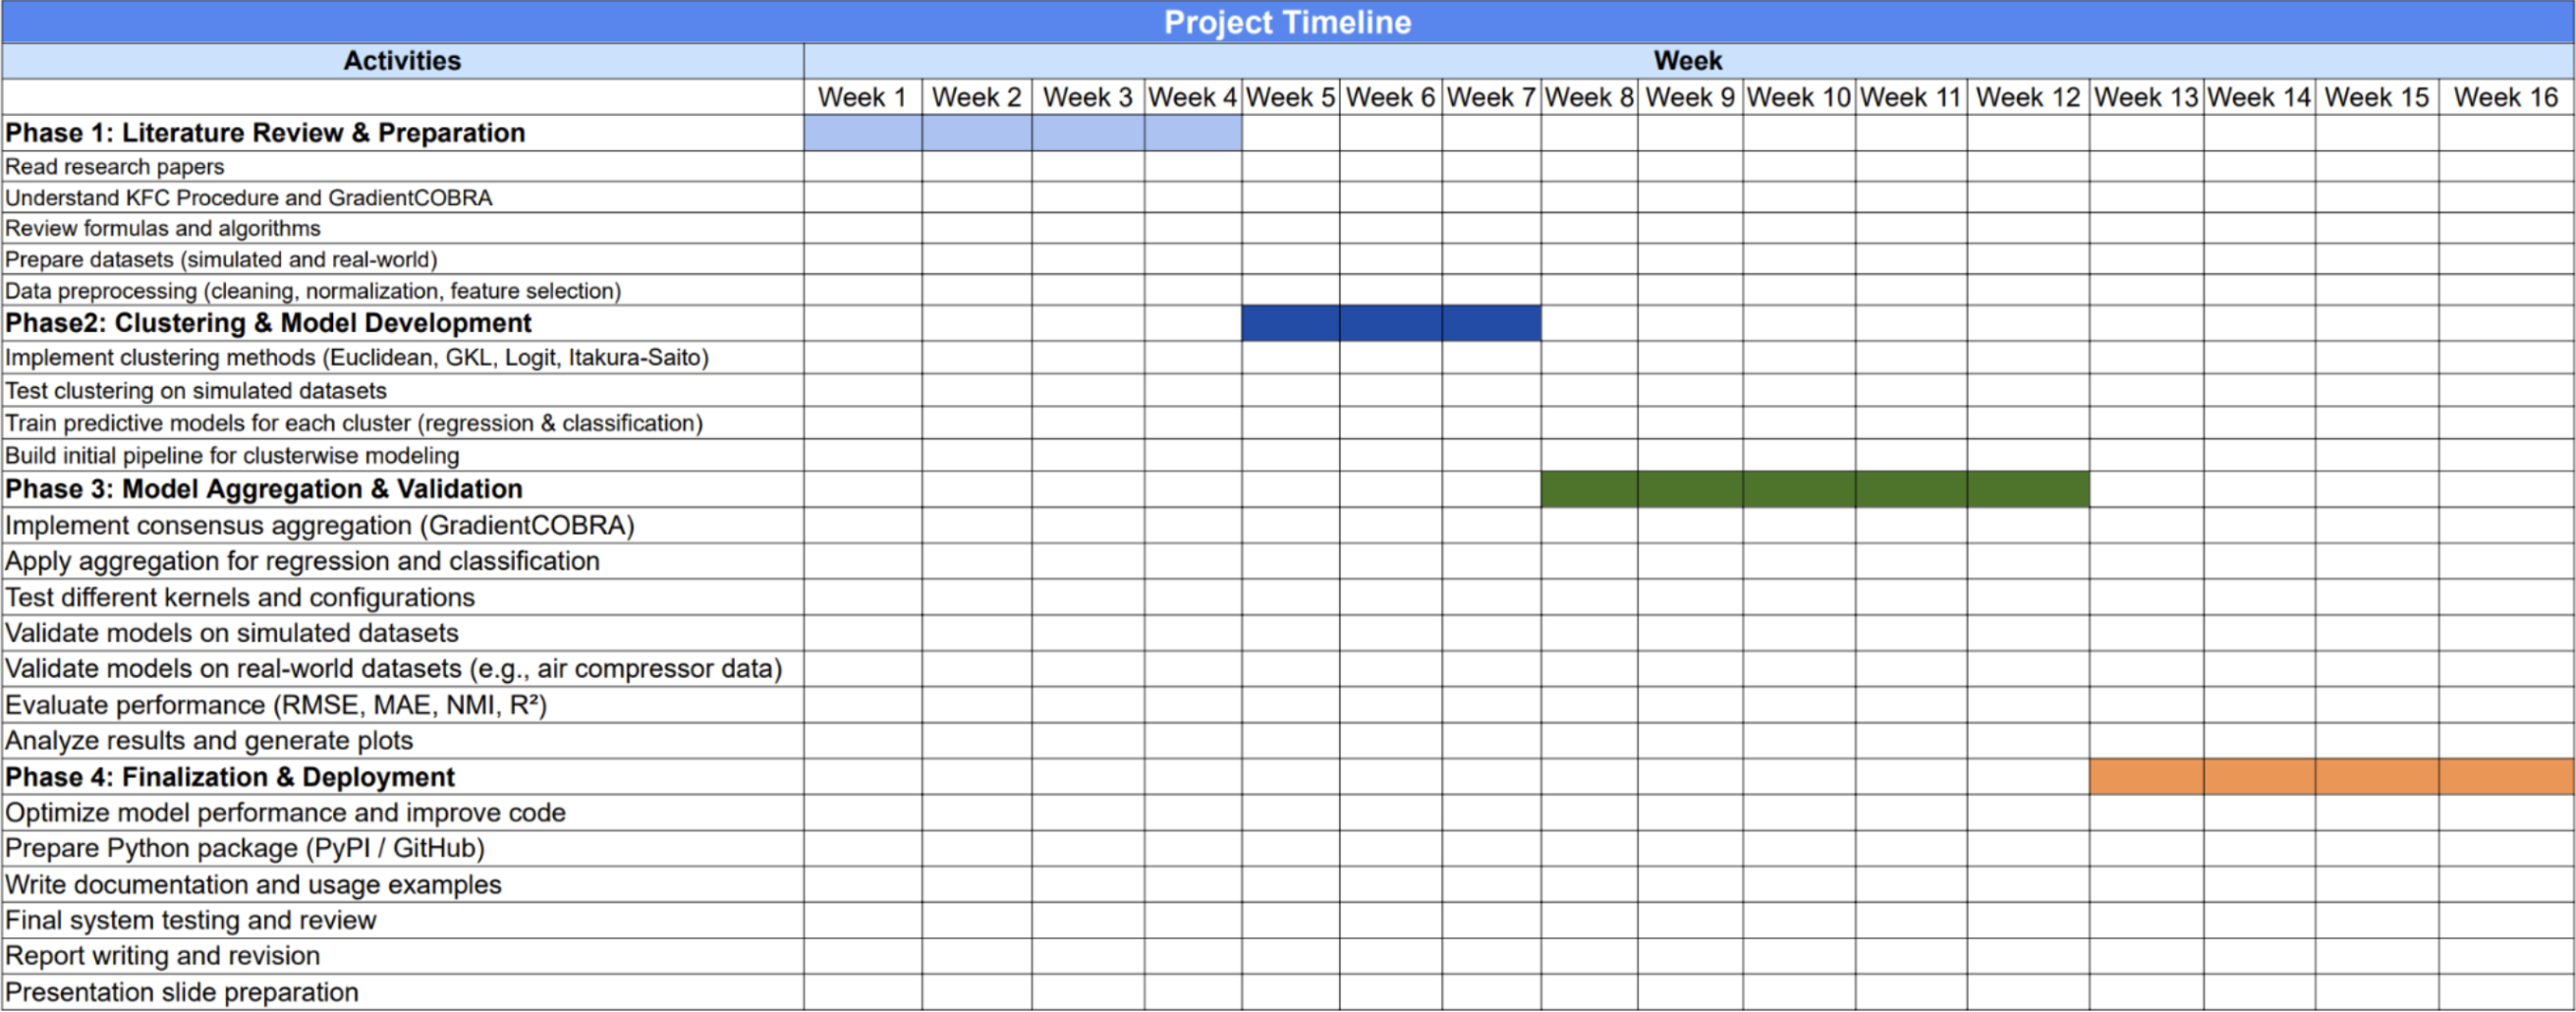
\includegraphics[width=0.8\textwidth]{figures/timeline.png}
    \caption{TimeLine}
    \label{fig:timeline}
\end{figure}